\documentclass{beamer}
\usepackage{ctex}
\usetheme{focus}

\title{算法分析与设计II}
\subtitle{2022-2023-2}
\date{Last Modified: 2023.1.16}
\institute{\vspace{2em} 数学与计算机学院 \\ 数据科学与大数据技术}
\titlegraphic{\vspace{5em} 
\includegraphics[scale=0.3]{fig/jlnu.pdf}}

\begin{document}

\frame{\titlepage}

\section{1. 课程说明}
\begin{frame}{教材与参考书}
    \begin{itemize}
        \item 教材
        \begin{itemize}
            \item《程序设计算法与实践》
        \end{itemize}
        \item 参考书
        \begin{itemize}
            \item 《ACM/ICPC算法训练教程》,余立功,清华大学出版社
            \item 《算法导论(原书第3版)》殷建平,等译,机械工业出版社
            \item 《算法竞赛》,罗勇军,等,清华大学出版社
            \item 《数据结构与算法分析—C语言描述(原书第2版)》冯舜玺 译,机械工业出版社
        \end{itemize}
    \end{itemize}
\end{frame}
\begin{frame}{参考慕课}
    \begin{itemize}
        \item 程序设计与算法(二)算法基础,郭炜,北京大学
        \item 慕课网址:
        \begin{itemize}
            \item https://www.bilibili.com/video/av45109397/
            \item 或 https://www.icourse163.org/course/PKU-1001894005
        \end{itemize}
        \item 慕课教材:
        \begin{itemize}
            \item 《算法基础与在线实践》,刘家瑛 等,高等教育出版社
        \end{itemize}
    \end{itemize}
\end{frame}
\begin{frame}{课程关系}
    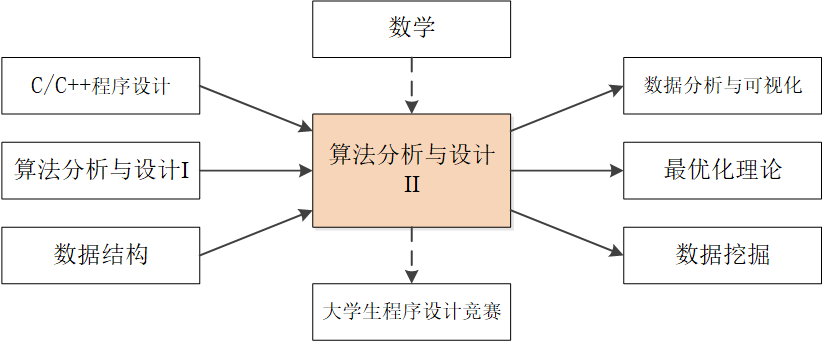
\includegraphics[scale=0.7]{fig/1-1.png}
\end{frame}
\begin{frame}{如何学习}
    \begin{itemize}
        \item 课前:
        \begin{itemize}
            \item 读教材例题英文原题(要讲到的例题必读,其他选读)
        \end{itemize}
        \item 课后:
        \begin{itemize}
            \item 学院OJ(做题量作为平时成绩): http://acm.jlnu.edu.cn
            \item 北大OJ(看Discuss): http://poj.org
            \item 自学扩展对应知识点
        \end{itemize}
        \item 成绩(\alert{考试课})
        \begin{itemize}
            \item 平时成绩:学院OJ做题量+其他(20\%)
            \item 期中测验+期末测验:学院OJ(80\%)
        \end{itemize}
    \end{itemize}
\end{frame}
\begin{frame}{主要内容}
    \begin{enumerate}
    \setcounter{enumi}{1}
        \item 基础算法
        \begin{itemize}
            \item 枚举法/递归法/分治法
        \end{itemize}
        \item 基础数据结构
        \begin{itemize}
            \item 堆栈/队列/堆
        \end{itemize}
        \item 动态规划
        \item 贪心算法
        \item 高级数据结构
        \begin{itemize}
            \item 并查集/线段树/树状数组/二叉搜索树/哈希表/字符串
        \end{itemize}
        \item 搜索算法
        \item 图算法
        \item 计算几何
    \end{enumerate}
\end{frame}



\end{document}